\section{Fonctions d'analyse}

	
	Comme précisé dans la {\sc Section} \ref{section:archi}, \glasir{} est constitué de trois modules principaux pour atteindre son objectif d'aide aux experts en sécurité. Ces modules proposent des fonctionnalités d'analyse des ADTrees qui seront détaillées dans cette section. 


	\subsection{Optimiseur}
		\label{subsection:optimiseur}

		Une fois que l'expert a obtenu son arbre complet avec ADTool (qui peut se composer de plusieurs milliers de nœuds), il ne peut pas facilement identifier le chemin optimal selon un paramètre donné. Il s'agit en effet d'un travail manuel, relativement fastidieux, qui doit être recommencé à chaque modification de l'arbre.
		
		Pourtant, la méthode utilisée est systématique. Il suffit de parcourir l'arbre en partant de la racine et de sélectionner à chaque étage le nœud le plus intéressant. Pouvoir identifier automatiquement le chemin optimal fera gagner beaucoup de temps à l'expert, et permettra aussi de limiter les risques d'erreurs. Ce processus peut donc être implémenté dans \glasir{}. 

		Nous allons donc créer un \textit{optimiseur} afin de répondre à ce besoin.
		Ses entrées seront les suivantes :
		\begin{itemize}
			\item un arbre provenant du projet ;
			\item le paramètre à prendre en compte.
		\end{itemize}
		Nous obtiendrons en sortie un nouvel arbre (qui sera un sous-graphe de l'arbre d'entrée), contenant le chemin optimal. L'expert pourra ensuite le traiter comme un tout nouvel arbre, en fonction de ses besoins.
		
		Prenons en exemple l'arbre de la {\sc Figure} \ref{fig:pre_optimiseur}. Si l'objectif est de trouver un chemin optimal avec le paramètre \og coût minimal \fg{}, et en critère la fonction $min$, on obtient l'arbre de la {\sc Figure} \ref{fig:arbre_post_opti}.
		
		\begin{landscape}
	        \begin{figure}
	            % \centering
	            \includegraphics[height=0.82\textwidth]{figure/pre_optimiseur.pdf}
	            \caption{L'arbre avant l'utilisation de l'optimiseur.}
	            \label{fig:pre_optimiseur}
	        \end{figure}
    	\end{landscape}		
		
		\begin{figure}[h!]
			\centering
			\includegraphics[width=0.35\textwidth]{figure/post_optimiseur.pdf}
			\caption{L'attaque optimale (par rapport au coût minimal) est ainsi facilement lisible.}
			\label{fig:arbre_post_opti}
		\end{figure}
	
		L'algorithme parcourant l'arbre à la recherche du chemin idéal est détaillé dans l'Algorithme \ref{algo:opti}.
		\begin{algorithm}[h!]
			\caption{opti(racine, param)}
			\label{algo:opti}
			\begin{algorithmic}
				\STATE l\_fils = fils(racine)
				\IF{vide(l\_fils)}
					\RETURN
				\ENDIF
				\STATE
				\IF{mode(racine) == ou}
					\STATE v = param(racine)

					\FOR{n in l\_fils}
						\IF{not defense(n) and param(n) != v}
							\STATE delete(n) // will delete subtrees as well
						\ENDIF
					\ENDFOR
				\ENDIF
				\STATE
				\FOR{n in fils(racine)}
					\STATE opti(n, param)
				\ENDFOR
			\end{algorithmic}
		\end{algorithm}
		Les notations non explicites sont présentées ci-dessous :
		\begin{itemize}
			\item \verb|racine| correspond au nœud à partir duquel nous élaguerons l'arbre ;
			\item \verb|param| est une fonction renvoyant une valeur pour un nœud donné ;
			\item \verb|fils| est une fonction renvoyant la liste des fils du nœud passé en paramètre ;
			\item \verb|defense| est une fonction prenant un nœud en entrée et renvoyant un booléen indiquant si il s'agit d'un nœud d'attaque ou de défense.
		\end{itemize}
		Il est récursif et modifie l'arbre en l'état (ce qui nous oblige de travailler sur une copie de l'arbre). 
		Ainsi, pour lancer l'optimisation, nous appellerons notre fonction \verb|opti| avec la racine de l'arbre en paramètre (il s'agit donc d'un parcours dit \og top-down \fg) . Dans le pire des cas, tous les nœuds seront à garder, et la complexité sera donc en $\mathcal{O}(n)$, $n$ étant le nombre de nœuds de l'arbre.

	\subsection{Filtre}
		\label{subsection:filtre} 

		Souvent, l'expert en sécurité va chercher à se défendre contre un attaquant précis. Dans ce cas, il va identifier les ressources dont l'attaquant dispose (temps, argent, etc.), pour ne conserver que les chemins de l'arbre empruntables par l'attaquant.

		Nous allons donc implémenter une fonctionnalité permettant de répondre à ce besoin, que nous appellerons \textit{filtre}. L'expert devra définir un critère selon lequel effectuer le filtrage, puis choisir un intervalle dans lequel les valeurs du paramètre devront se situer. Il sera possible de filtrer l'arbre selon plusieurs paramètres à la fois.

		Les entrées de la fonction de filtrage seront donc les suivantes :
		\begin{itemize}
			\item l'arbre à filtrer ;
			\item les valuations de l'arbre servant de critères pour le filtrage ;
			\item les intervalles de sélection sur les différentes valuations.
		\end{itemize}
		L'arbre retourné par la fonction de filtrage sera une copie élaguée de l'arbre original. Seuls les chemins respectant tous les intervalles de filtrage seront conservés.

		Par exemple, en appliquant un filtre sur l'intervalle $[0, 500]$ et sur la valuation \og coût minimal \fg{} à l'arbre de la {\sc Figure} \ref{fig:arbre_post_opti}, on obtient l'arbre de la {\sc Figure} \ref{fig:arbre_post_filtre}, qui contient uniquement des valeurs comprises dans l'intervalle spécifié. 
		\begin{figure}[!h]
			\begin{center}
				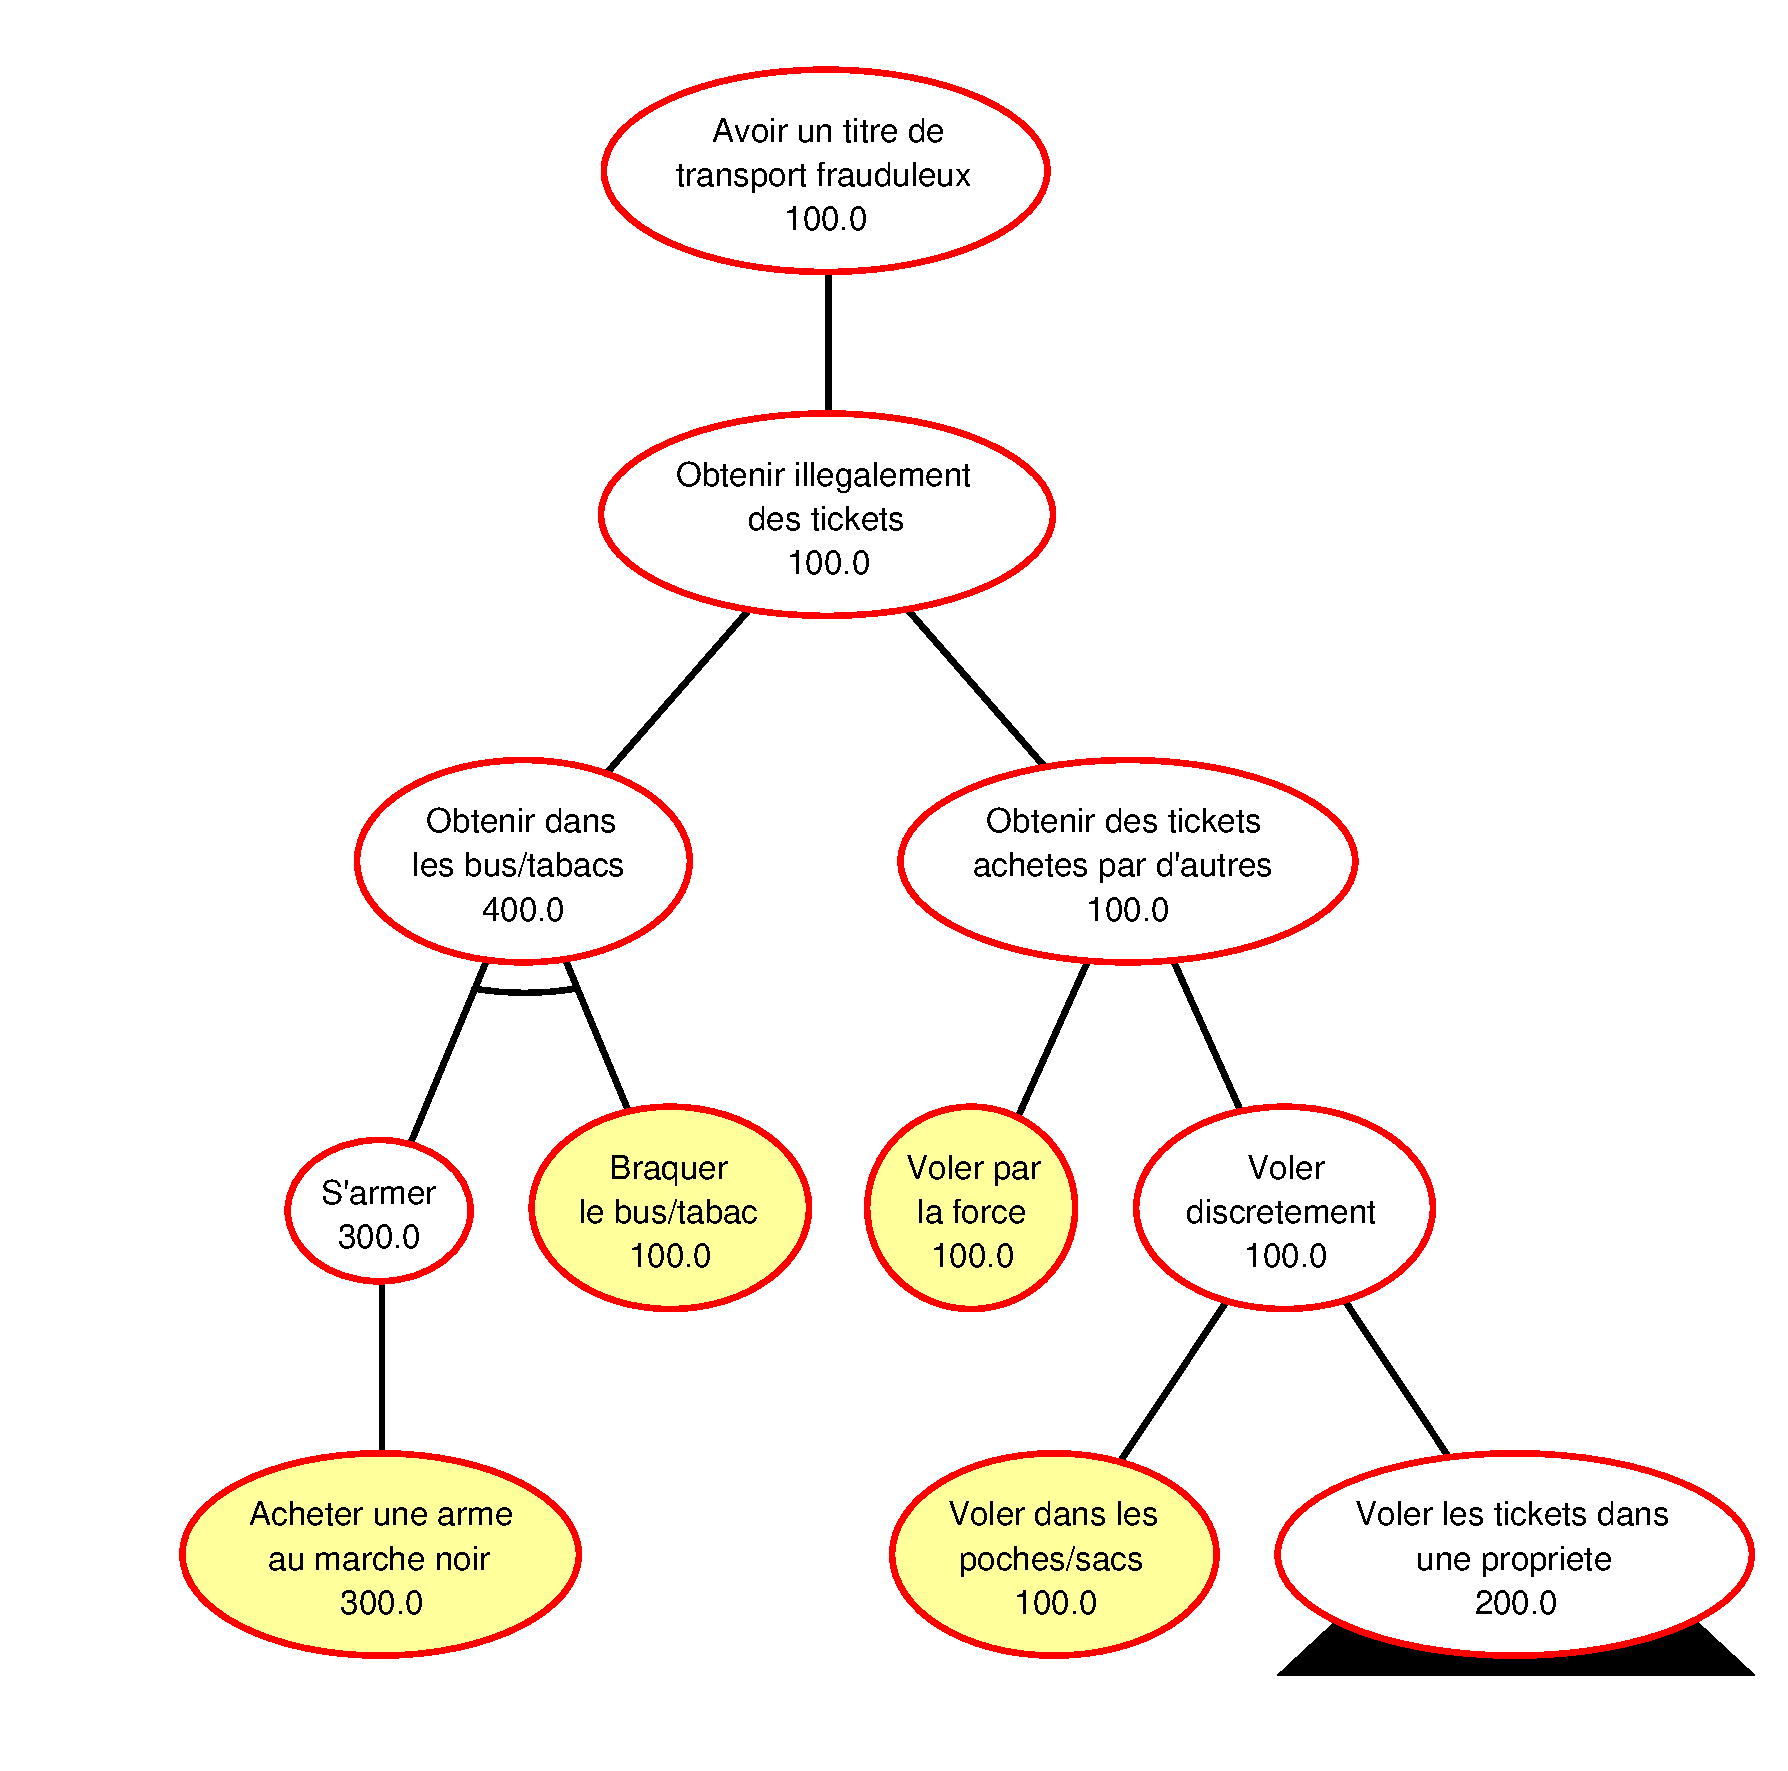
\includegraphics[width=0.75\textwidth]{figure/post_filtre.pdf}
			\end{center}
			\caption{Arbre filtré selon le coût minimal pour l'attaquant.}
			\label{fig:arbre_post_filtre}
		\end{figure}
		On constate que l'arbre élagué par le filtre a été considérablement réduit. L'arbre exemple étant de très petite taille comparé aux modélisations de systèmes réels, on comprend bien l'utilité de cette fonctionnalité pour l'expert.

		Nous utiliserons dans ce module l'Algorithme \ref{algo:filtre}. 
		\begin{algorithm}[h!]
			\caption{filtre(racine, rules)}
			\label{algo:filtre}
			\begin{algorithmic}
				\FOR{r in rules}
					\IF{not r(racine)}
						\STATE delete(racine AND subtrees)
						\RETURN
					\ENDIF
				\ENDFOR
				\STATE
				\FOR{n in fils(racine)}
					\STATE filtre(n, rules)
				\ENDFOR
			\end{algorithmic}
		\end{algorithm}
		Il est lui aussi récursif, le nombre d'appels sera donc au pire en $\mathcal{O}(n)$.
		\begin{itemize}
			\item \verb|racine| est le point de départ de l'algorithme ;
			\item \verb|rules| est l'ensemble des règles de filtrage (valuations et intervalles).
		\end{itemize}
	

		\subsection{Éditeur de fonctions}
			\label{subsection:synthese} 

			L'expert est actuellement cantonné aux paramètres présentés dans la {\sc{Section}} \ref{sec:adtool} et ne peut pas en créer d'autres, ce qui limite ses possibilités d'analyse. En effet, les paramètres déjà existants ne sont pas les seuls pouvant intéresser un expert en sécurité. Nous souhaitons donc rendre possible la création de nouveaux paramètres, à partir de ceux déjà disponibles et des fonctions mathématiques de base (division, multiplication, min, max, etc.). Ces nouvelles valuations pourront ensuite être appliquées à n'importe quel arbre, de la même manière que les paramètres de base. Elles pourront ainsi être utilisées pour évaluer les arbres selon de nouveaux critères, et si besoin pour les élaguer à l'aide du filtre que nous allons implémenter.

			Cette nouvelle fonctionnalité prendra donc en entrée les éléments suivants :
			\begin{itemize}
				\item un arbre provenant du projet courant ;
				\item les paramètres intervenant dans la synthèse ;
				\item les opérations mathématiques appliquées ;
				\item le nom du paramètre de synthèse généré.
			\end{itemize}

			\paragraph{}
			Par exemple, dans l'arbre de la {\sc{Figure}} \ref{fig:pre_optimiseur}, nous pouvons voir que les deux sous-arbres \og Obtenir illégalement des tickets \fg{} (sous-arbre A) et \og Falsifier des tickets \fg{} (sous-arbre B) permettent d'atteindre l'objectif final. Il est actuellement possible de les valuer par treize paramètres, nous n'en garderons ici que deux pour simplifier : le coût minimal et la probabilité de succès.

			On constate rapidement que choisir A implique un coût de réalisation moindre pour l'attaquant, puisqu'il nécessite peu de matériel. Cependant, un vol est toujours risqué, et les chances de se faire arrêter sont élevées, diminuant fortement la probabilité de succès. Opter pour le sous-arbre B, bien que plus cher à réaliser, permet de limiter ce risque et d'augmenter la probabilité de succès. On voit donc que ces deux paramètres, qui ne sont pas liés, peuvent être tous les deux utiles à l'expert et entraîner deux interprétations très différentes. C'est pourquoi il serait intéressant de pouvoir les combiner, grâce à notre éditeur de fonctions, afin de les prendre en compte simultanément. C'est ensuite à l'expert de juger des liens qu'il désire instaurer entre les paramètres : fonctions mathématiques, coefficients, etc. Par exemple, s'il décide d'appeler le nouveau paramètre \og result \fg{}, et qu'il estime qu'il s'agit du coût auquel on ajoute la probabilité de succès multipliée par deux, on obtient la synthèse suivante : \[ result = (minimal\_cost) + 2 \times (probability\_of\_success).\]
			La synthèse \og result \fg{} sera désormais disponible pour donner des valuations aux nœuds, et pourra elle-même être utilisée pour créer d'autres paramètres.

			Les principaux modules de \glasir{} étant présentés, la prochaine section détaillera l'implémentation de différentes fonctionnalités dans \glasir{} pour le rendre simple et pratique. De plus, elle traitera des améliorations apportées à ADToool pour le rendre plus ergonomique pour l'utilisateur.
